\section{Auswertung}
\label{sec:Auswertung}

\subsection{Empfindlichkeit der Braunschen Röhre}
Um die Empfindlichkeit $\frac{D}{U_\mathrm{d}}$ zu ermitteln, wird für die sieben Messreihen (siehe Tabelle \ref{tab:messwerte1}) bei unterschiedlichen Beschleunigugsspannungen $U_\mathrm{B}$ jeweils die Auslenkung $D$ gegen die Ablenkspannung $U_\mathrm{d}$ aufgetragen. Mittels einer linearen Ausgleichsrechnung wird die Steigung der Geraden der Form $y=ax+b$, welche der Empfindlichkeit entspricht, bestimmt. Dargestellt ist dies in den Abbildungen \ref{fig:empfindlichkeit1} und \ref{fig:empfindlichkeit2}.

\begin{table}
\centering
  \caption{Messwerte zu $U_\mathrm{d}$ und $D$ bei verschiedenen $U_\mathrm{B}$.}
  \label{tab:messwerte1}
\scalebox{0.69}{
  \begin{tabular}{c c c}
    \toprule
    $U_\mathrm{B}/ \si{\volt}$ & $D/\si{\meter}$ & $U_\mathrm{d}/\si{\volt}$\\
    \midrule
200 & -0,0254 & -20,43 \\
200 &-0,01905 & -16,85 \\
200 & -0,0127 & -13,44 \\
200 & -0,00635 & -9,64 \\
200 & 0 & -6,15 \\
200 & 0,00635 & -2,49 \\
200 & 0,0127 & 1,22 \\
200 & 0,01905 & 4,98 \\
200 & 0,254 & 7,89 \\
250 & -0,0254 & -25,50 \\
250 &-0,01905 & -21,59 \\
250 & -0,0127 & -16,95 \\
250 & -0,00635 & -12,29 \\
250 & 0 & -7,76 \\
250 & 0,00635 & -3,24 \\
250 & 0,0127 & 1,24 \\
250 & 0,01905 & 6,19 \\
250 & 0,254 & 10,51 \\
300 & -0,0254 & -30,40 \\
300 &-0,01905 & -25,03 \\
300 & -0,0127 & -20,04 \\
300 & -0,00635 & -14,72 \\
300 & 0 & -9,19 \\
300 & 0,00635 & -3,90 \\
300 & 0,0127 & 1,84 \\
300 & 0,01905 & 7,92\\
300 & 0,0254 & 13,27 \\
350 & -0,0238125 & -33,96 \\
350 &-0,01905 & -29,50 \\
350 & -0,0127 & -23,85 \\
350 & -0,00635 & -17,05 \\
350 & 0 & -10,79 \\
350 & 0,00635 & -4,46 \\
350 & 0,0127 & 2,49 \\
350 & 0,01905 & 8,49 \\
350 & 0,0254 & 15,36 \\
400 & -0,0206375 & -34,60 \\
400 &-0,01905 & -32,82 \\
400 & -0,0127 & -26,18 \\
400 & -0,00635 &-19,28 \\
400 & 0 &-12,26 \\
400 & 0,00635 &-5,24 \\
400 & 0,0127 & 2,15 \\
400 & 0,01905 & 9,66 \\
400 & 0,0254 &16,76 \\
450 & -0,015875 & -33,85 \\
450 &-0,0142875 & 31,38 \\
450 & -0,0127 & -26,69 \\
450 & -0,00635 & -21,80 \\
450 & 0 & -13,89 \\
450 & 0,00635 & -5,87 \\
450 & 0,0127 & 2,32 \\
450 & 0,01905 & 10,37 \\
450 & 0,0254 & 18,93 \\
500 & -0,0142875 & -34,52 \\
500 &-0,0127 & 32,93 \\
500 & -0,009525 & -28,12 \\
500 & -0,00635 & -23,72 \\
500 & 0 & -15,33 \\
500 & 0,00635 & -6,46 \\
500 & 0,0127 & 2,57 \\
500 & 0,01905 & 12,02 \\
500 & 0,0254 & 21,21 \\
\bottomrule
\end{tabular}
}
\end{table}

\begin{figure}
  \centering
  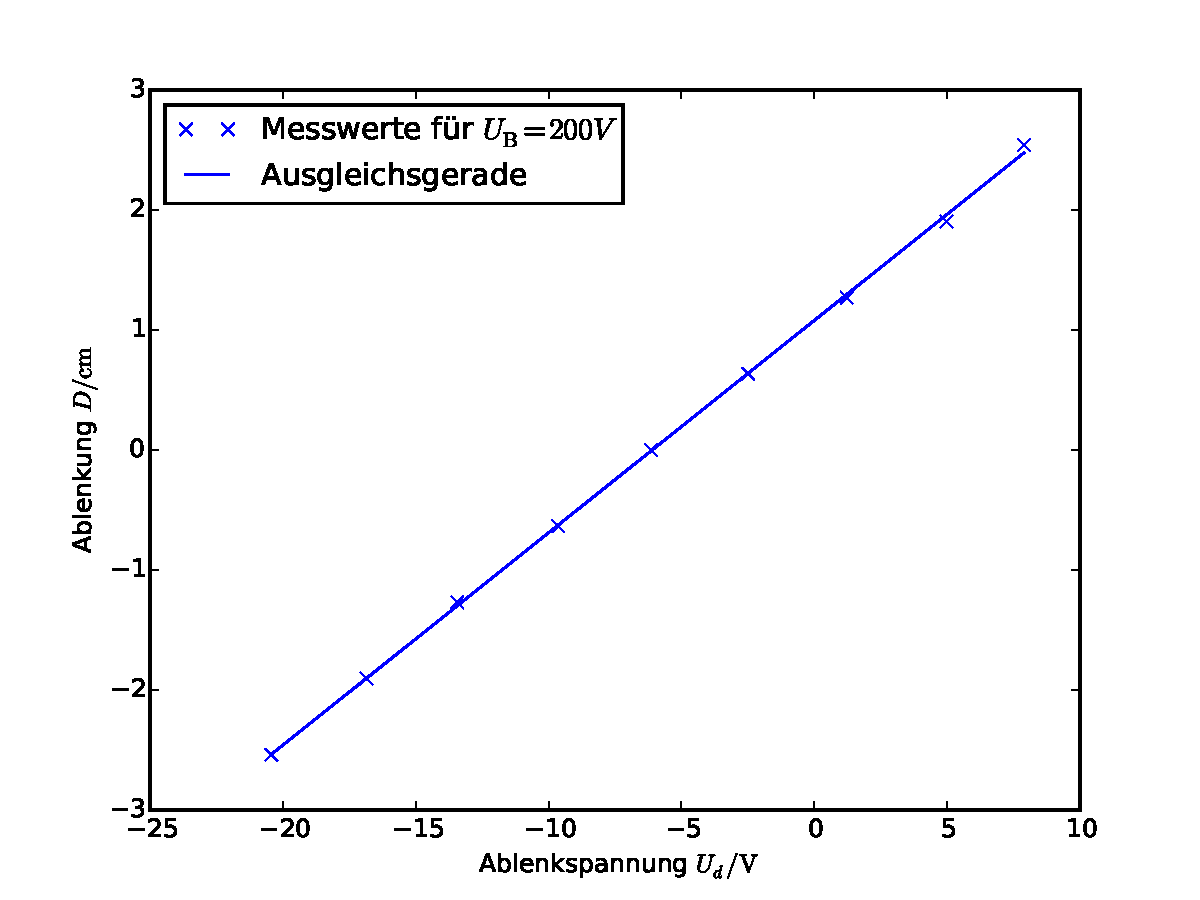
\includegraphics[scale=0.8]{auswertung/501-a1.pdf}
\caption{Ablenkung $D$ in Abhängigkeit von $U_\mathrm{d}$ für $U_\mathrm{B}$ 200 - 350 \si{\volt}.}
  \label{fig:empfindlichkeit1}
\end{figure}

\begin{figure}
  \centering
  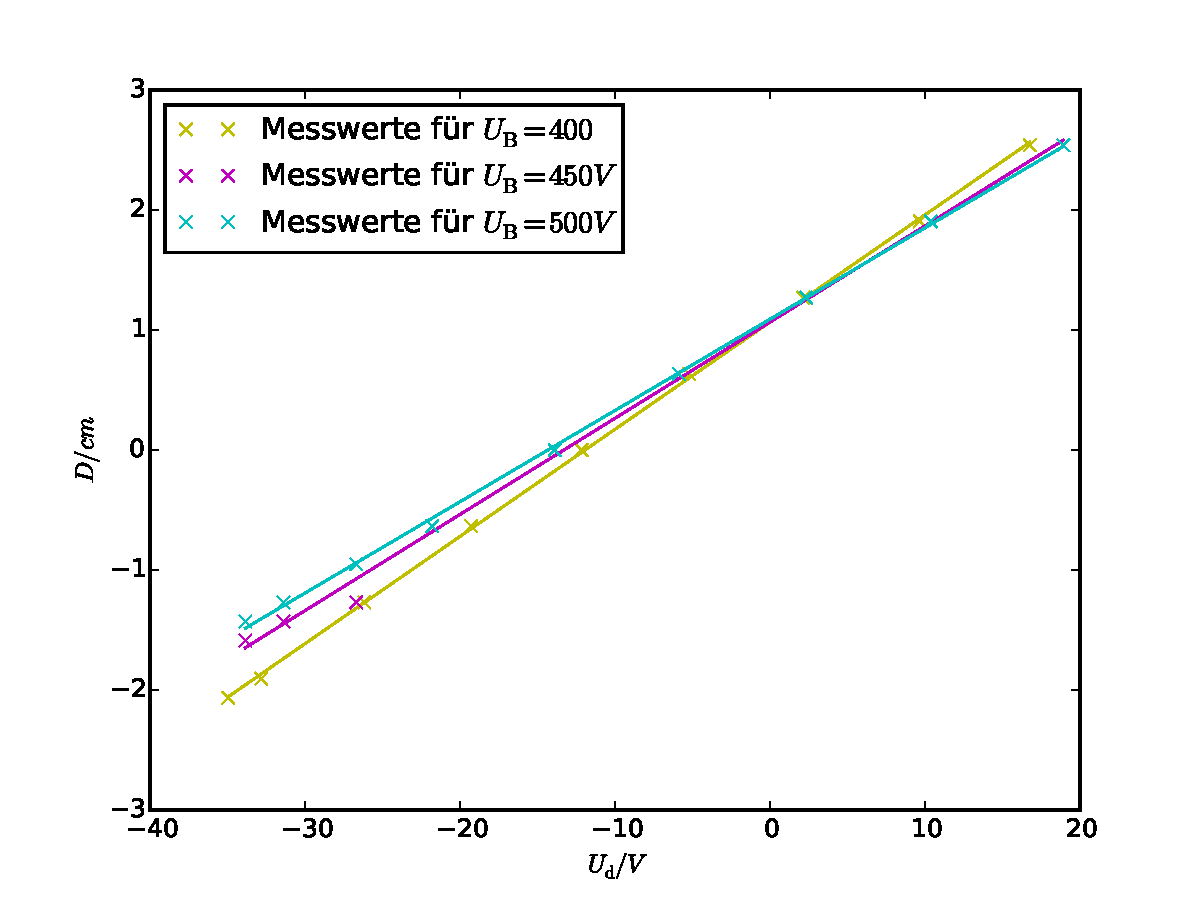
\includegraphics[scale=0.8]{auswertung/501-a2.pdf}
\caption{Ablenkung $D$ in Abhängigkeit von $U_\mathrm{d}$ für $U_\mathrm{B}$ 400 - 500 \si{\volt}.}
  \label{fig:empfindlichkeit2}
\end{figure}

Die berechneten Werte für Die Steigung und den y-Achsenabschnitt der Geraden befinden sich in Tabelle \ref{tab:empfindlichkeit}.

\begin{table}
  \caption{Werte für die Steigungen der Ausgleichsgeraden.}
  \centering
  \label{tab:empfindlichkeit}
  \begin{tabular}{c c c}
    \toprule
    $U_\mathrm{B} / \si{\volt}$ & $\frac{D}{U_\mathrm{d}}/ 10^{-2} \frac{\si{\meter}}{\si{\volt}}$ & $b / 10^{-2}\si{\meter}$ \\
    \midrule
200 & 0,177 \pm 0,001 & 1,078 \pm 0,014 \\
250 & 0,140 \pm 0,001 & 1,077 \pm 0,012 \\
300 & 0,116 \pm 0,001 & 1,035 \pm 0,017 \\
350 & 0,099 \pm 0,001 & 1,048 \pm 0,015 \\
400 & 0,089 \pm 0,001 & 1,066 \pm 0,011 \\
450 & 0,080 \pm 0,002 & 1,066 \pm 0,034 \\
500 & 0,076 \pm 0,001 & 1,090 \pm 0,015 \\
\bottomrule
\end{tabular}
\end{table}

Damit ergibt sich für die Empfindlichkeit gemittelt $\frac{D}{U_\mathrm{d}}=(0.0100 \pm 0.0004)10^{-2}\frac{\si{\meter}}{\si{\volt}}$.

\subsection{Bestimmung der Apparaturkonstante}
Die zuvor bestimmten Empfindlichkeiten sollen nun gegen $\frac{1}{U_\mathrm{B}}$ aufgetragen werden(siehe Abbildung \ref{fig:A}). erneut wird mittels linearer Ausgleichrechung die Steigung bestimmt und soll mit der Konstante $A=\frac{pL}{2d}$ verglichen werden.

\begin{figure}
  \centering
  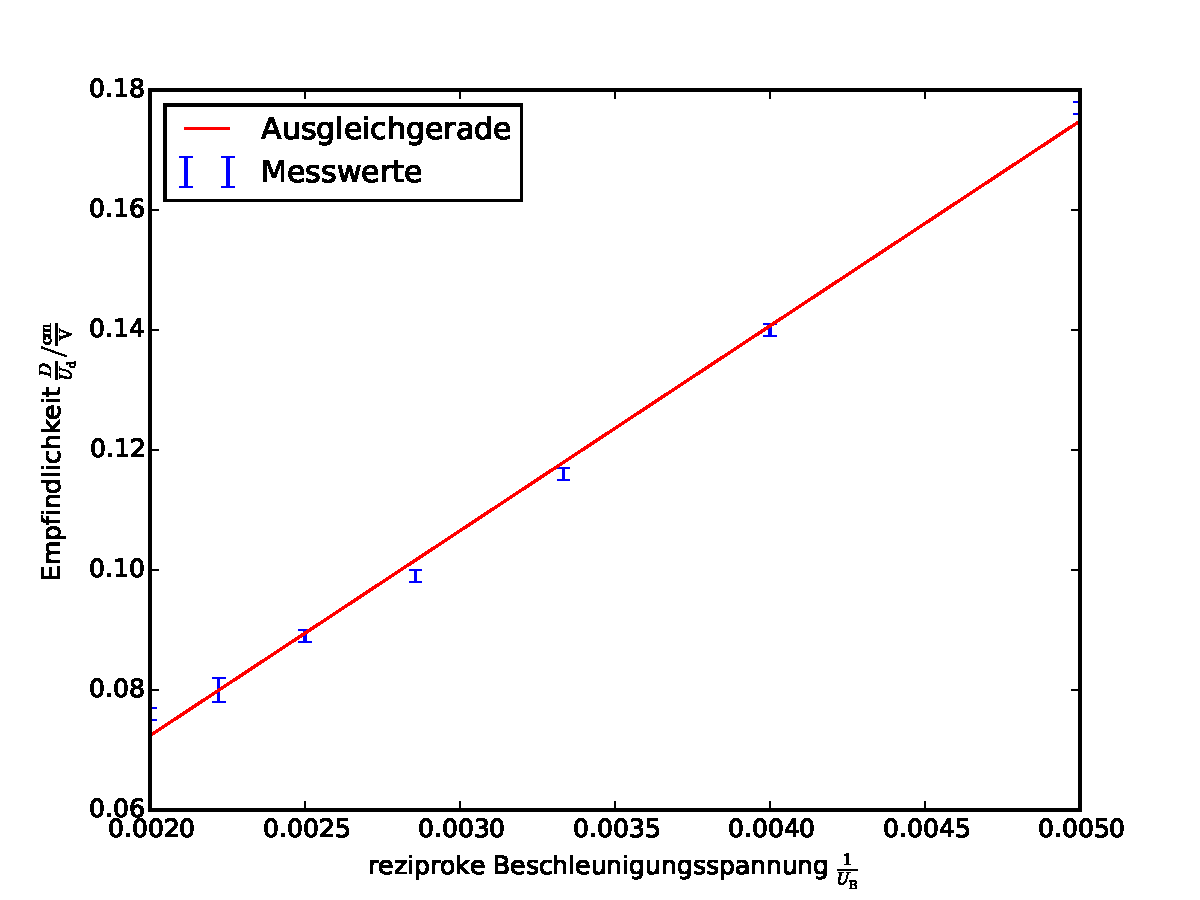
\includegraphics[scale=0.8]{auswertung/501-a3.pdf}
\caption{$\frac{D}{U_\mathrm{d}}$ in Abhängigkeit von $\frac{1}{U_\mathrm{B}}$ .}
  \label{fig:A}
\end{figure}

Für die Gerade gilt erneut $y=ax+b$. Für $a$ und $b$ ergeben sich folgende Werte:
\begin{align}
  a&=(34,147 \pm 0,972)10^{-2}\si{\meter}\\
  b&=(0,004 \pm 0,003)\frac{10^{-2}\si{\meter}}{\si{\volt}}\\
\end{align}
Mit
\begin{align}
  p&=0,0019 \si{\meter}\\
  l&=0,143 \si{\meter} \\
  d&=0,00038 \si{\meter}\\
\end{align}
ergibt sich für $A=0,3575$ \si{\meter}. Das entspricht einer Abweichung von $(4,7 \pm 3)\%$ zur berechneten Steigung der Ausgleichsgeraden.

\subsection{Kathodenstrahl-Oszillograph}
Im folgenden Teil soll aus den vier gemessenen Frequenzen der Sägezahnspannung die Frequenz der anliegenden Sinusspannung ermittelt sowie ih Scheitelwert berechnet werden. Die gemessenen Frequenzen befinden sich in Tabelle \ref{tab:frequenzen}.

\begin{table}
  \caption{Werte für die Steigungen der Ausgleichsgeraden.}
  \centering
  \label{tab:frequenzen}
  \begin{tabular}{c c}
    \toprule
    $f / \si{\Hz}$ & $D/\si{\meter}$ \\
    \midrule
79,87 & 0,01905 \\
39,95 & 0,01905\\
159,75 & 0,01905 \\
239,37 & 0,01905 \\
\bottomrule
\end{tabular}
\end{table}

Mit der Synchronisationsbedingung $n f_\mathrm{Sä}= m f_\mathrm{sin}$ folgt, dass $f_\mathrm{sin}=79,87$ \si{\Hz}.
Setzt man die Empfindlichkeit mit $\frac{D}{U_\mathrm{sin}}$ gleich, erhält man.
\begin{equation}
  (0.0100 \pm 0.0004)10^{-2}\frac{\si{\meter}}{\si{\volt}} = \frac{0,1905 \si{\meter}}{U_\mathrm{sin}}
\Rightarrow U_\mathrm{sin} = 190,5 \si{\volt}.
\end{equation}

\subsection{Ablenkung der Elektronen im Magnetfeld}
Die gemessenen Spulenströme für verschiedene Beschleunigungsspannungen sind in Tabelle \ref{tab:messwerte2} dargestellt. Das $B$-Feld innerhalb der Spule kann mit Formel \eqref{eqn:spule} berechnet werden. Nun soll, wie in Abbildung \ref{fig:spez.ladung1} und \ref{fig:spez.ladung2} dargestellt, $\frac{D}{L^2+D^2}$ gegen $B$ aufgetragen werden und aus der Steigung der Ausgleichsgeraden die spezifische Ladung $\frac{e}{m_\mathrm{e}}$ bestimmt werden.

\begin{table}
  \caption{Messwerte zu $U_\mathrm{d}$, und $D$ bei verschiedenen $U_\mathrm{B}$.}
  \centering
  \label{tab:messwerte2}
  \begin{tabular}{c c c}
    \toprule
    $U_\mathrm{B}/ \si{\volt}$ & $D/\si{\meter}$ & $I_\mathrm{s}/\si{\ampere}$\\
    \midrule
250 & 0 & 0 \\
250 & 0,0254 & 0,27 \\
250 & 0,0508 & 0,60 \\
250 & 0,0762 & 0,91 \\
250 & 0,1016 & 1,25 \\
250 & 0,127 & 1,58 \\
250 & 0,1524 & 1,91 \\
250 & 0,1778 & 2,25 \\
250 & 0,2032 & 2,59 \\
300 & 0  & 0 \\
3000 & 0,0254 &0,32 \\
300 & 0,0508 & 0,67 \\
300 & 0,0762 & 1,04 \\
300 & 0,1016 & 1,38 \\
300 & 0,127 & 1,75 \\
300 & 0,1524 & 2,09 \\
300 & 0,1778 & 2,45 \\
300 & 0,2032 & 2,81 \\
350 & 0  & 0 \\
350 & 0,0254 & 0,33 \\
350 & 0,0508 & 0,70\\
350 & 0,0762 & 1,09 \\
350 & 0,1016 & 1,47 \\
350 & 0,127 & 1,84 \\
350 & 0,1524 & 2,27 \\
350 & 0,1778 &2,68 \\
350 & 0,2032 & 3,02 \\
400 & 0  & 0 \\
400 & 0,0254 & 0,4 \\
400 & 0,0508 & 0,77 \\
400 & 0,0762 & 1,22 \\
400 & 0,1016 & 1,63 \\
400 & 0,127 & 2,05 \\
400 & 0,1524 & 2,49 \\
400 & 0,1778 & 2,88 \\
400 & 0,2032 & / \\
450 & 0  & 0 \\
450 & 0,0254 & 0,41 \\
450 & 0,0508 & 0,82 \\
450 & 0,0762 & 1,28 \\
50 & 0,1016 & 1,69 \\
450 & 0,127 & 2,12 \\
450 & 0,1524 & 2,58 \\
450 & 0,1778 & 3,01 \\
450 & 0,2032 & / \\
\bottomrule
\end{tabular}
\end{table}

\begin{figure}
  \centering
  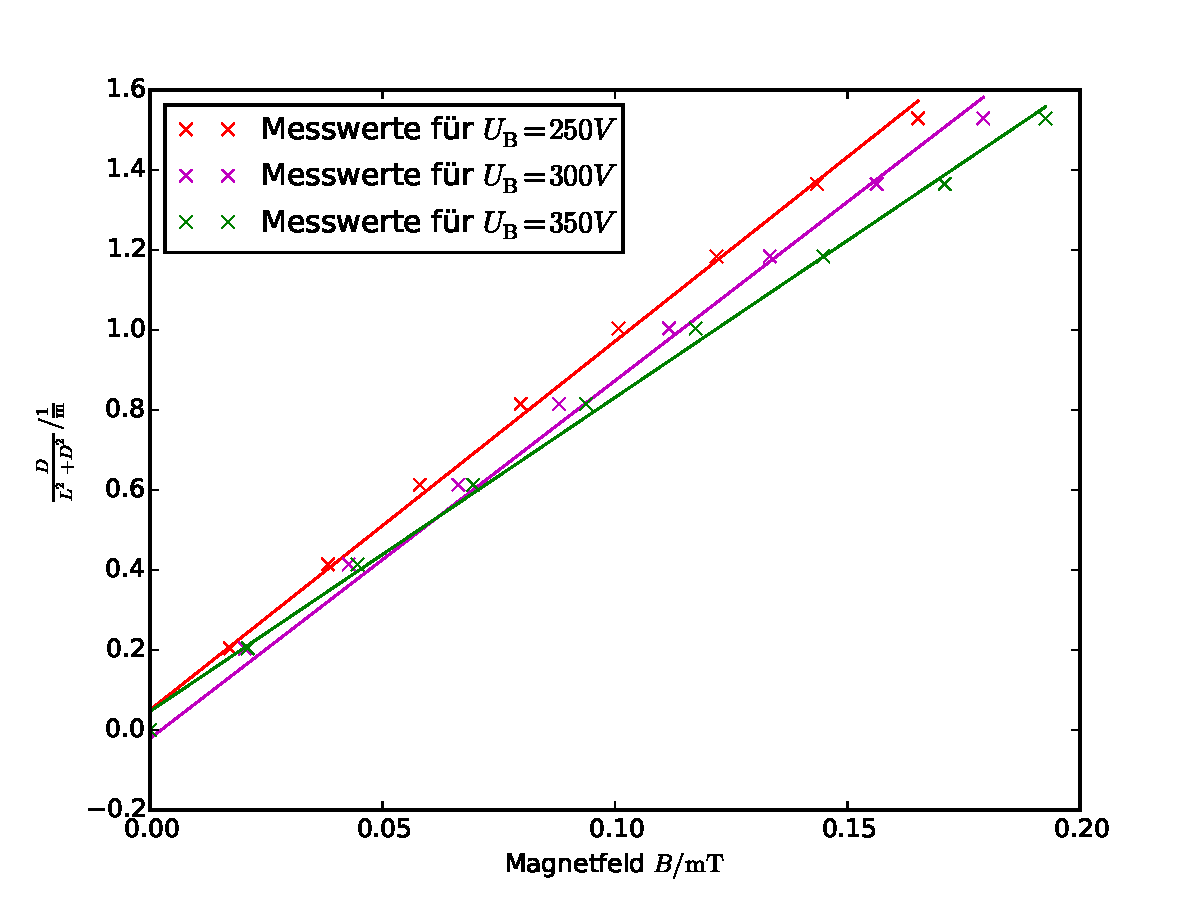
\includegraphics[scale=0.8]{auswertung/502-a.pdf}
\caption{$\frac{D}{L^2+D^2}$ in Abhängigkeit von $B$ für $U_\mathrm{B} 250 - 350 \si{\volt}$.}
  \label{fig:spez.ladung1}
\end{figure}

\begin{figure}
  \centering
  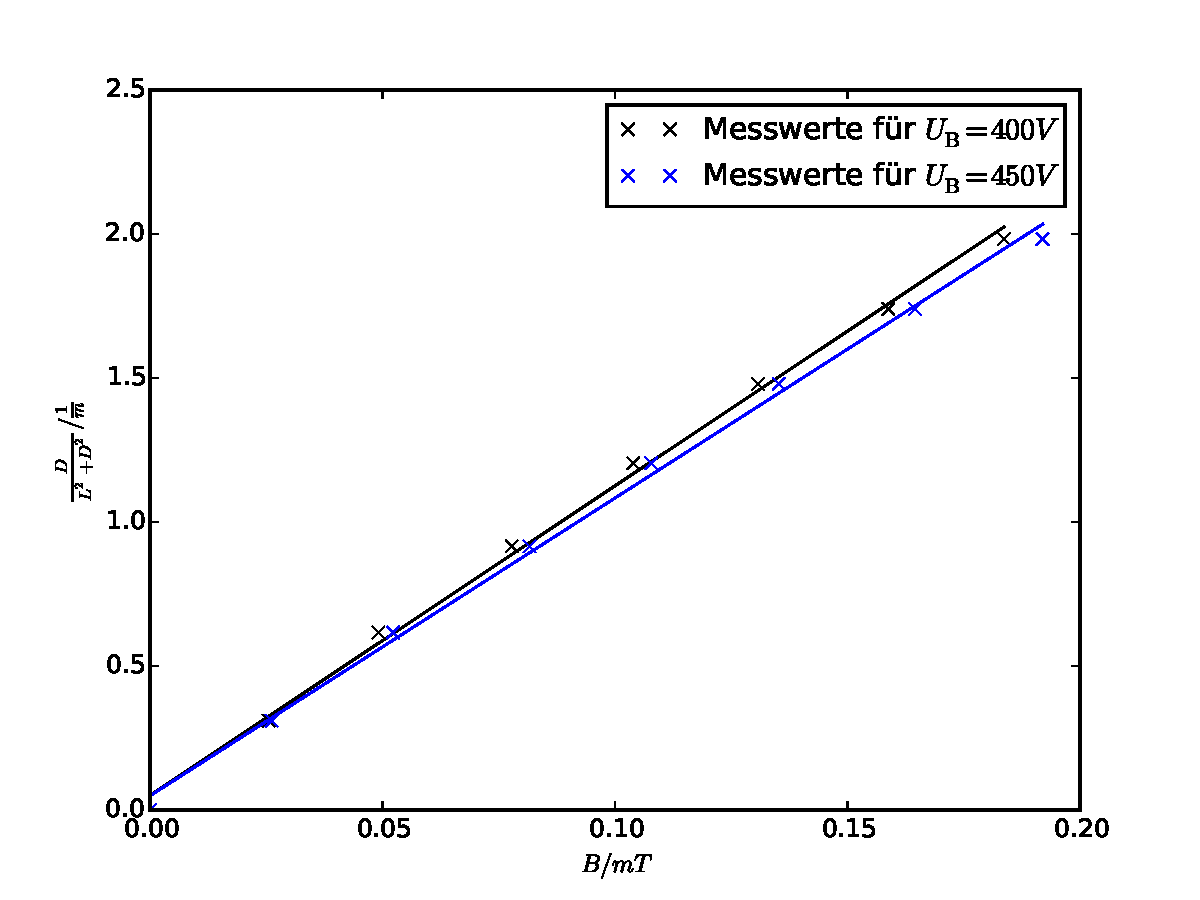
\includegraphics[scale=0.8]{auswertung/502-a2.pdf}
\caption{$\frac{D}{L^2+D^2}$ in Abhängigkeit von $B$ für $U_\mathrm{B} 400 - 500 \si{\volt}$.}
  \label{fig:spez.ladung2}
\end{figure}

Für alle geraden gilt $y=ax+b$. Die Werte der Parameter für die Ausgleichsgeraden befinden sich in Tabelle \ref{tab:spez.ladung}.
Mit Gleichung \eqref{eqn:spez} folgt für die spezifische Ladung
\begin{equation}
  \frac{e}{m_\mathrm{e}}=8U_\mathrm{B}a^2.
\end{equation}
Die Werte hierzu befinden sich ebenfalls in \ref{tab:spez.ladung}.

\begin{table}
  \caption{Werte für die Steigungen der Ausgleichsgeraden und die daraus ermittelte spezifische Ladung.}
  \centering
  \label{tab:spez.ladung}
  \begin{tabular}{c c c c}
    \toprule
     $U_\mathrm{B} / \si{\volt}$ & $a/ \frac{1}{\si{\meter\milli\tesla}}$ & $b / \frac{1}{\si{\meter}}$ & $\frac{e}{m_\mathrm{e}}/\frac{\si{\coulomb}}{\si{\kilo\gram}}10^9$ \\
    \midrule
250 & 13,308 \pm 0,366 & 0,090 \pm 0,035 & 11,1 \pm 1,8  \\
300 & 12,323 \pm 0,274 & 0,069 \pm 0,029 & 8,4 \pm 1,1 \\
350 & 11,326 \pm 0,001 & 0,086 \pm 0,035 &5,9 \pm 0,9\\
400 & 10,745 \pm 0,226 & 0,051 \pm 0,025 & 4,9 \pm 0,6\\
450 & 10,339 \pm 0,220 & 0,049 \pm 0,025 & 4,4 \pm 0,6\\
\bottomrule
\end{tabular}
\end{table}

Damit ergibt sich für die spezifische Ladung ein Mittelwert von $\frac{e}{m_\mathrm{e}}=(6,9 \pm 0,5)10^9 \frac{\si{\coulomb}}{\si{\kilo\gram}}$.

\subsection{Bestimmung der Totalintensität des Erdmagnetfeldes}
Für den Spulestrom und dem Inklinationswinkel werden folgende Werte gemessen:
\begin{align}
  I_\mathrm{hor}&=0,12 \si{\ampere}\\
  \phi &= 72,5^\circ \\
\end{align}

Es wird erneut Gleichung \eqref{eqn:spule} für das $B$-Feld innerhalb einer Helmholtzspule verwendet. Mit der gemessenen Stromstärke ergibt sich die Horizontalkomponente des Erdmagnetfeldes. Für die Totalintensität gilt
\begin{equation}
  B_\mathrm{total}=\frac{B_\mathrm{hor}}{\cos(\phi)}.
\end{equation}
Damit ergibt sich $B_\mathrm{total}=2.54 \cdot 10^{-5}\si{\tesla}$.
